\subsection{一致空间的紧性}

定义 2 一致空间 X 称为准紧的，如果它的 Hausdorff 完备化 \(\hat{\mathbf{X}}\) 是紧的。一致空间 X 的子集 A 称为准紧子集，如果 X 的一致子空间 A 是准紧的。

于是，一致空间 X 的子集 A 是准紧的，当且仅当 \(i(\mathbf{A})\) 在 \(\hat{X}\) 中的闭包是紧的（ \(i: X \rightarrow \hat{X}\) 为典范映射）（ \(\S\) 3 第 9 目命题 18 推论 1）。

例。在任何一致空间 X 中，Cauchy 序列 \((x_{n})\) 的点组成的集是准紧的。由于诸 \(x_{n}\) 在 \(\hat{X}\) 中的像仍构成 Cauchy 序列，我们可以假定 X 是 Hausdorff 的；于是在 \(\hat{X}\) 中，由诸点 \(x_{n}\) 组成的集的闭包由诸点 \(x_{n}\) 与 \(\lim_{n\to\infty}x_{n}\) 组成，因而是紧的（第一章 § 9 第 3 目例 2）。

定理 3 一致空间 X 是准紧的，当且仅当对 X 的每个一致邻域 V，存在 X 的一个由 V-小集组成的有限覆盖。

我们可以更直观地把这个条件表述为：X 可以被有限多个集覆盖，而这些集要多么小就可以多么小。

设 \(i: \mathbf{X} \to \hat{\mathbf{X}}\) 为典范映射，则 \(\mathbf{X}\) 的一致邻域是经由 \(i \times i\) 从 \(\hat{\mathbf{X}}\) 的一致邻域取逆像而得的集合（§ 3 第 7 目命题 12）。设 \(\mathbf{X}\) 准紧，并设 \(\mathbf{U}\) 为任一一致邻域（\(\hat{\mathbf{X}}\) 的）；则存在一个对称一致邻域 \(\mathbf{U}'\)（\(\hat{\mathbf{X}}\) 的），使 \(\hat{\mathbf{U}}' \subset \mathbf{U}\)。由于 \(\hat{\mathbf{X}}\) 是紧的，存在有限多个点 \(x_j \in \hat{\mathbf{X}}\) 使诸 \(\mathbf{U}'(x_j)\)（它们是 U-小集）覆盖 \(\hat{\mathbf{X}}\)。若 \(\mathbf{V}\) 是 \(\mathbf{U}\) 经由 \(i \times i\) 的逆像，则诸集合 \(i^{-1}(\mathbf{U}'(x_j))\) 是 V-小集且覆盖 \(\mathbf{X}\)。反之，假设对每个一致邻域 \(\mathbf{V}\)（\(\mathbf{X}\) 的），存在 \(\mathbf{X}\) 的一个由 V-小集组成的有限覆盖。我们要证明每个超滤子 \(\mathfrak{F}\)（\(\hat{\mathbf{X}}\) 上的）都收敛；由于 \(\hat{\mathbf{X}}\) 是完备的，只需证明 \(\mathfrak{F}\) 是 Cauchy 滤子，即对每个闭一致邻域 \(\mathbf{U}\)（\(\hat{\mathbf{X}}\) 的），在 \(\mathfrak{F}\) 中有一个 U-小集（§ 1 第 2 目命题 2 推论 2）。设 \(\mathbf{V}\) 是 \(\mathbf{U}\) 在 \(i \times i\) 下的逆像，并设 \((\mathbf{B}_j)\) 是 \(\mathbf{X}\) 的一个由 V-小集组成的有限覆盖；则诸集合 \(C_j = i(B_j)\) 是 U-小集且覆盖 \(i(\mathbf{X})\)，于是

\[
\hat {\mathbf {X}} = \bigcup_ {j} \overline {{\mathbf {C}}} _ {j}.
\]

另一方面，由于 \(\mathbf{C}_j \times \mathbf{C}_j \subset \mathbf{U}\)，且 \(\mathbf{U}\) 在 \(\hat{\mathbf{X}} \times \hat{\mathbf{X}}\) 中是闭的，故 \(\overline{\mathbf{C}}_j \times \overline{\mathbf{C}}_j \subset \mathbf{U}\)，从而诸 \(\overline{\mathbf{C}}_j\) 也是 \(\mathbf{U}\)-小集。由于 \(\mathfrak{F}\) 是超滤子，诸 \(\overline{\mathbf{C}}_j\) 之一属于 \(\mathfrak{F}\)（第一章 § 6 第 4 目命题 5 的推论）。

证毕。

推论 一致空间 X 是紧的，当且仅当它是 Hausdorff 的、完备的，并且能被有限多个 V-小集覆盖，其中 V 是 X 的任一一致邻域。

这由定理 3 及第 1 目的定理 1 得出。

注 1 非 Hausdorff 的拟紧空间未必可一致化，因为它未必满足公理 (O \(_{III}\) )（参看第一章 § 9 第 2 目）；例如代数几何中出现的大多数非 Hausdorff 拟紧空间都不满足公理 (O \(_{III}\) )（参看习题 2）。

命题 1 在一致空间中，准紧集的每个子集、准紧集的每个有限并以及每个准紧集的闭包都是准紧的。

前两个断言是定理 3 的直接推论。设 X 是一致空间，A 是 X 的准紧子集，并设 \(i: \mathbf{X} \to \hat{\mathbf{X}}\) 为典范映射。\(i(\overline{\mathbf{A}})\) 包含在 \(i(\mathbf{A})\) 于 \(\hat{\mathbf{X}}\) 中的闭包内（第一章 § 2 第 1 目定理 1），因此 \(i(\overline{\mathbf{A}})\) 在 \(\hat{\mathbf{X}}\) 中的闭包包含在一个紧集中，从而是紧的。

\pandocbounded{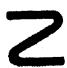
\includegraphics[keepaspectratio]{images/part002_3e3611b3.jpg}}

注 2 在一致空间 X 中，相对紧集 A 是准紧的，因为 A 包含在一个紧集中。另一方面，即使 X 是 Hausdorff 的，准紧集也未必在 X 中相对紧，X 本身准紧但不紧的情形就表明了这一点。

命题 2 设 \(f: \mathbf{X} \to \mathbf{Y}\) 是一致连续映射。若 \(\mathbf{A}\) 是 \(\mathbf{X}\) 的任一准紧子集，则 \(f(\mathbf{A})\) 是 \(\mathbf{Y}\) 的准紧子集。因为若 \(i: \mathbf{X} \to \hat{\mathbf{X}}\) 与 \(j: \mathbf{Y} \to \hat{\mathbf{Y}}\) 为典范映射，我们有 \(j(f(\mathbf{A})) = \hat{f}(i(\mathbf{A}))\)（§ 3 第 7 目命题 15），因而 \(j(f(\mathbf{A}))\) 在 \(\hat{\mathbf{Y}}\) 中相对紧（第一章 § 9 第 4 目定理 2 推论 1）。

命题 3 设 X 是一个集合，\((\mathrm{Y}_{\lambda})_{\lambda \in \mathbf{L}}\) 是一族一致空间，且对每个 \(\lambda \in L\)，设 \(f_{\lambda}\) 是 X 到 \(Y_{\lambda}\) 中的映射。设 X 赋有使诸 \(f_{\lambda}\) 一致连续的最粗一致结构。则 X 的子集 A 是准紧的，当且仅当 \(f_{\lambda}(A)\) 是 \(Y_{\lambda}\) 的准紧子集（对每个 \(\lambda \in L\)）。

这个条件由命题 2 知是必要的。充分性由 § 3 第 9 目命题 18 给出的 X 的 Hausdorff 完备化的刻画以及 Tychonoff 定理（第一章 § 9 定理 3 的推论）得出。

